% Packages

\documentclass[
	11pt, % Set the default font size, options include: 8pt, 9pt, 10pt, 11pt, 12pt, 14pt, 17pt, 20pt
	%t, % Uncomment to vertically align all slide content to the top of the slide, rather than the default centered
	%aspectratio=169, % Uncomment to set the aspect ratio to a 16:9 ratio which matches the aspect ratio of 1080p and 4K screens and projectors
]{beamer}
\setcounter{tocdepth}{1}
\usepackage{graphicx}
\usepackage[export]{adjustbox}
\graphicspath{{Images/}{./}} % Specifies where to look for included images (trailing slash required)
\usepackage{tikz}

\usepackage{booktabs} % Allows the use of \toprule, \midrule and \bottomrule for better rules in tables
\usepackage{pgfplots}
\usepackage{tikz}
\pgfplotsset{width=6cm, compat=newest, every tick label/.append style={scale=0.5}}

% Theme
\usetheme{Madrid}

% Font
\usefonttheme{serif}
\usepackage{newtxtext,newtxmath}
\usepackage[default]{lato}

% Inner theme
\useinnertheme{circles}

% Information
\title{Number systems and sets}
\author{Kin Hei Wong}
\date{\today}
%%%%%%%%%%%%%%%%%%%%%%%%%%%%%%%%%%%%%%%%%%%%%%%%%%%%%%%%%%
\begin{document}

% Title slide
\begin{frame}
    \titlepage
\end{frame}

% Table of Content
\begin{frame}
    \frametitle{Presentation overview}
    \tableofcontents
\end{frame}
%%%%%%%%%%%%%%%%%%%%%%%%%%%%%%%%%%%%%%%%%%%%%%%%%%%%%%%%%%%
% Body slides

\section{2A: Set notation}
\begin{frame}
    \frametitle{2A}
    \begin{center}
        \title{Set notation}
        \maketitle
    \end{center}
\end{frame}

\begin{frame}{General Notations}
    Before we begin, we must understand the following Mathematical Notations:
    \begin{enumerate}
        \item $\mathbb{N}$ - Natural number (1 to $\infty$)
        \item $\mathbb{Z}$ - Integers (No decimals)
        \item $\mathbb{Q}$ - Rational number (Recurring or non-infinity decimals)
        \item $\mathbb{R}$ - Real numbers (Numbers that includes rational and irrationals)
        \item $\mathbb{C}$ - Complex number (Numbers involves with $i$)
    \end{enumerate}
\end{frame}

\begin{frame}{Set notation}
    One of the simplest way to represent a whole set of number is by Venn diagram! It pictures out the summary of the case.\\
    The case is known as \textbf{disjoint}, such that in A and B have no elements in common.\\
    \begin{center}
        \includegraphics[width=0.5\textwidth]{disjoint.png}
    \end{center}
    We also create the sets like the following statement: E.g. A = {-3, 3} = {$x: x^2=9$}\\
    This example, {$x: ...$} is read as 'the set of all $x$ such that...'.
\end{frame}

\begin{frame}{Set notation}
    \begin{enumerate}
        \item $\in$ - is an element of (3 $\in$ Odd number)
        \item $\not\in$ - not an element of
        \item $=$ - if they contain same elements (if A = ${1,2,3}$, and also B = ${1,2,3, \text{then} A=B}$)
        \item $\emptyset$ - if a set has no element
        \item $\xi$ - contains all elements which are being considered
        \item $\subset$ - when some elements are contained in one other set (B = ${a,b,c}$, A = ${a,b}$, $\therefore$ A$\subset$B)
    \end{enumerate}
\end{frame}

\begin{frame}[t]
    \frametitle{Union ($\cup$), intersect ($\cap$) and complement (')}
    Find A$\cup$B, A$\cap$B, A', B', A'$\cup$B, A$\cap$B'.\\
    \begin{center}
        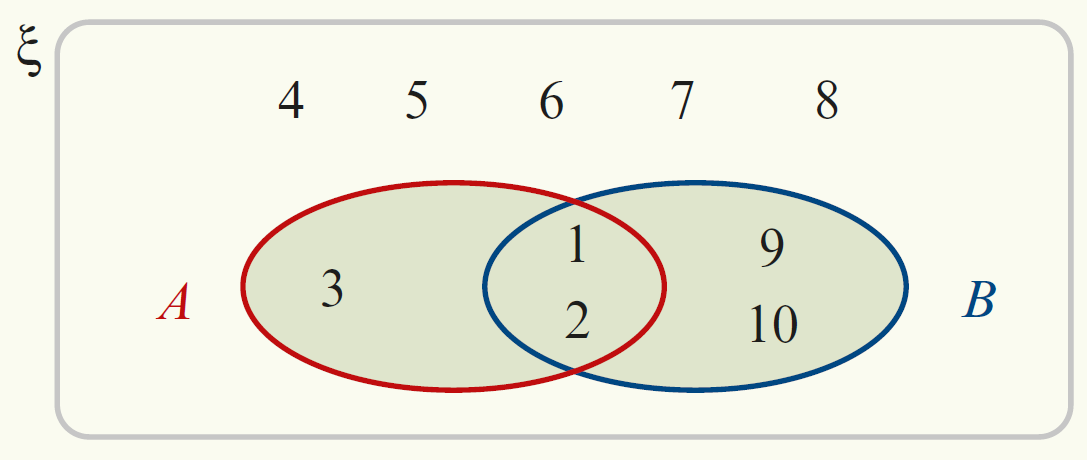
\includegraphics[width=0.5\textwidth]{Venn.png}       
    \end{center}
\end{frame}

\begin{frame}{Finite and infinite sets}
    The things mentioned previously were all finite sets, it ends at a point. However, there can be infinite sets too, where
     it is endless! \\(A = set of real number, $\mathbb{R}$)
\end{frame}

\begin{frame}{Exercise 2A}
\end{frame}
%%%%%%%%%%%%%%%%%%%%%%%%%%%%%%%%%%%%%%%%%%%%%%%%%%%%%%%%%%%%%%%
\section{2B: Sets of numbers}
\begin{frame} 
    \frametitle{2B}
    \begin{center}
        \title{Sets of numbers}
        \maketitle
    \end{center}
\end{frame}

\begin{frame}{Sets of numbers}
    As mentioned, there are infinite sets, such that it can be represented in $\mathbb{R}, \mathbb{Z}$, and etc.\\
    It is clear that $\mathbb{N} \subseteq \mathbb{Z} \subseteq \mathbb{Q} \subseteq \mathbb{R}$
    \begin{center}
        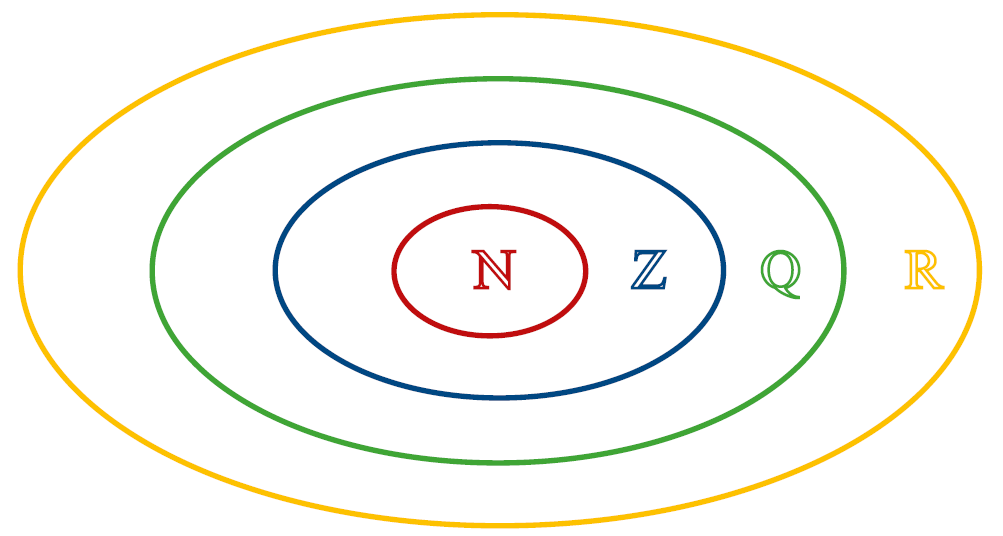
\includegraphics[width=0.3\textwidth]{Venn2.png}
    \end{center}
    There are other examples, such as:
    \begin{enumerate}
        \item ${x: 0<x<1}$
        \item ${x: x\geq 3}$
        \item ${2n: n\in \mathbb{Z}}$
    \end{enumerate}
    The set of all ordered pairs of real numbers is denoted by $\mathbb{R}^2$. That is,\\
    $\mathbb{R}^2 = {(x,y): x, y \in \mathbb{R}}$\\
    This set is known as the \textbf{Catersian product} of $\mathbb{R}$ with itself.
\end{frame}

\begin{frame}[t]
    \frametitle{Rational number}
    \begin{block}{Theorem}
        Every rational number can be written as a terminating or recurring decimal.
    \end{block}
    Proof: 
\end{frame}

\begin{frame}[t]
    \frametitle{Rational number}
    \begin{block}{Theorem}
        A real number has a terminating decial representation if and only if it can written as\\
        $\dfrac{m}{2^\alpha \times 5^\beta}$\\
        for some $m \in \mathbb{Z}$ and some $\alpha, \beta \in \mathbb{N} \cup {0}$.
    \end{block}
    Proof: 
\end{frame}

\begin{frame}[t]
    \frametitle{Rational number}
    \begin{block}{Example}
        Write each of the following in the form $\dfrac{m}{n}$, where $m$ and $n$ are integers:\\
        \begin{enumerate}[a]
            \item $0.05$
            \item $0.\dot{4}28571\dot{1}$
        \end{enumerate}
    \end{block}
\end{frame}
\begin{frame}
\end{frame}

\begin{frame}
    \frametitle{Real numbers}
    Made up of two importent subsets: \textbf{algebraic numbers, transcendental numbers}.
    Algebraic number - a solution to a polynomial equation of the form\\
    $a_nx^n + a_{n-1}x^{n-1} + ... + a_1x+a_0 = 0$, where $a_0, a_1, ..., a_n$ are integers\\
    All rational numbers is algebraic!\\
    \bigskip
    The irrational number $\sqrt{2}$ is algebraic, as it is a solution of the equation $x^2 - 2 = 0.$\\
    But $\pi$ is not! It is a transcendental number. Proof is too difficult to be given here.
\end{frame}

\begin{frame}
    \frametitle{Interval notation}
    \begin{center}
        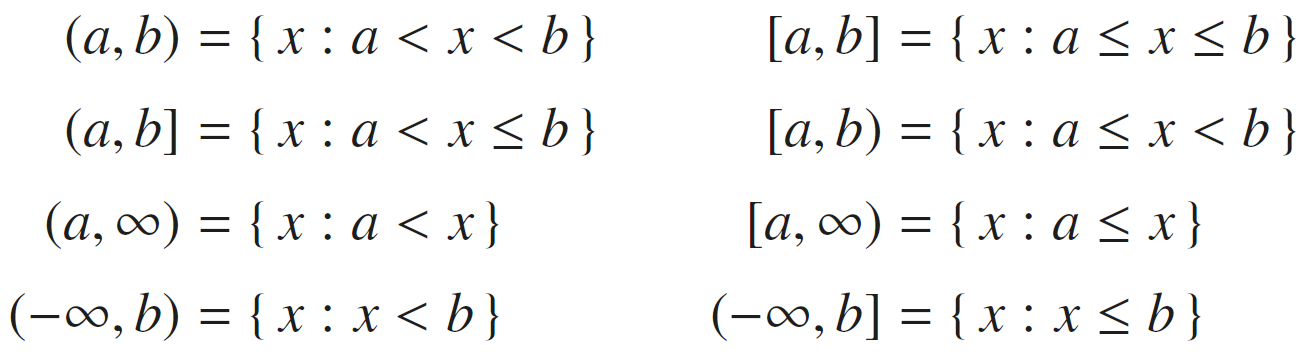
\includegraphics[width=0.7\textwidth]{Interval.png}\\
    \end{center}
    The following are subsets of the real numbers for which we have special notation:\\
    \begin{enumerate}
        \item $\mathbb{R}^+ = {x: x>0}$
        \item $\mathbb{R}^- = {x: x<0}$
        \item Real numbers excluding zero: $\mathbb{R}\setminus$$\{0\}$
    \end{enumerate}
\end{frame}
\begin{frame}{Exercise 2B}
\end{frame}
%%%%%%%%%%%%%%%%%%%%%%%%%%%%%%%%%%%%%%%%%%%%%%%%%%%%%%%%%%%%%%%
\section{2C: Surds}
\begin{frame} 
    \frametitle{2C}
    \begin{center}
        \title{Surds}
        \maketitle
    \end{center}
\end{frame}

\begin{frame}{Before introducing surds...}
    We need to understand the properties of square roots:\\
    \begin{block}{Properties of square roots}
        \begin{enumerate}
            \item $\sqrt{ab} = \sqrt{a}\sqrt{b}$
            \item $\sqrt{\frac{a}{b}} = \frac{\sqrt{a}}{\sqrt{b}}$
        \end{enumerate}
    \end{block}
\end{frame}

\begin{frame}{Intro. to surds!}
    \begin{block}{What is a surd?}
        In general, a \textbf{surd of order n} is a number of the form $\sqrt[n]{a}$, where $a$ is a rational number which is \alert{not} a perfect
        $n$th power.
    \end{block}
    But we are mainly focusing on quadratic surd, where n = 2.\\
    \bigskip
    \begin{block}{Why is surd important?}
        We can expect to see surds as an exact solution (without converting to decimals), such as in trig.\\
        $sin(60^\circ) = \frac{\sqrt{3}}{2}$, \quad $sin(15^\circ) = \frac{\sqrt{6} - \sqrt{2}}{4}$
    \end{block}
\end{frame}

\begin{frame}[t]
    \frametitle{Example}
    Write each of the following in simplest form:\\
    \begin{enumerate}
        \item $\sqrt{72}$
        \item $\sqrt{28}$
        \item $\sqrt{\frac{700}{117}}$
        \item $\sqrt{\frac{99}{64}}$
    \end{enumerate}
\end{frame}

\begin{frame}{Like surds}
    Surds which have the same 'irrational factor' are \textbf{like surds}.\\
    E.g. $3\sqrt{7}, 2\sqrt{7}, \sqrt{7}$ have factor of $\sqrt{7}$, $\therefore$ it is like surds.\\
    \begin{block}{Properties of like surds}
        \begin{enumerate}
            \item $m\sqrt{p} + n\sqrt{p} = (m+n)\sqrt{p}$
            \item $m\sqrt{p} - n\sqrt{p} = (m-n)\sqrt{p}$
        \end{enumerate}
    \end{block}
\end{frame}

\begin{frame}[t]
    \frametitle{Example}
    \begin{enumerate}
        \item $\sqrt{147} + \sqrt{108} - \sqrt{363}$
        \item $\sqrt{3} + \sqrt{5} + \sqrt{20} + \sqrt{27} - \sqrt{45} - \sqrt{48}$
        \item $\sqrt{50} + \sqrt{2} - 2\sqrt{18} + \sqrt{8}$
    \end{enumerate}
\end{frame}

\begin{frame}[t]
    \frametitle{Rationalising the \textbf{denominator}}
    Rationalising - a method to keep the surds clean and tidy\\
    \begin{block}{Example}
        \begin{enumerate}
            \item $\frac{1}{2\sqrt{7}}$
            \item $\frac{1}{2 - \sqrt{3}}$
            \item $\frac{1}{\sqrt{3} - \sqrt{6}}$
            \item $\frac{3 + \sqrt{8}}{3 - \sqrt{8}}$
        \end{enumerate}
    \end{block}
\end{frame}
\begin{frame}    
\end{frame}

\begin{frame}{Exercise 2C}
\end{frame}
%%%%%%%%%%%%%%%%%%%%%%%%%%%%%%%%%%%%%%%%%%%%%%%%%%%%%%%%%%%%%%%
\section{2D: Natural numbers}
\begin{frame} 
    \frametitle{2D}
    \begin{center}
        \title{Natural numbers}
        \maketitle
    \end{center}
\end{frame}

\begin{frame}{Factors and composites}
    Factors:\\
    Let $a$ be natural number, and it is a factor of number $b$, then there exists a natural number $k$, where $b = ak$.\\
    \alert{E.g. factor of 8: 1, 2, 4, 8}\\
    Composite:\\
    Let $m$ be composite number if it can be written as a product of $m = a \times b$, where $a, b$ are natural numbers
    greater than 1 and less than $m$\\
    \alert{E.g. 12 is a composite number because: $12 = 4 \times 3 = 2^2 \times 3$}\\

    \begin{block}{What are their differences?}
        In short:\\
        Factor: natural number(s) that can divide the number you are investigating\\
        Composites: natural number that can change to a group of numbers multiplying\\
    \end{block}
\end{frame}

\begin{frame}{Prime decomposition}
    Prime number: natural number greater than 1 and if its only factor of itself and 1.\\
    Basically, we break down the composite number into group of prime numbers multiplying.\\
    \begin{block}{Fundamental theorem of arithmetic}
        Fundamental Theorem of Arithmetic states that every integer greater than 1 is either a prime number or can be expressed in the form of primes. 
        In other words, all the natural numbers can be expressed in the form of the product of its prime factors.
    \end{block}
\end{frame}

\begin{frame}[t]
    \frametitle{Example}
    Give the prime decomposition of 17248, and hence list the factors of this number.    
\end{frame}

\begin{frame}{Highest common factor(HCF) vs Lowest common multiple(LCM)}
    \begin{block}{HCF or Greater common divisor (GCF)}
        The highest common factor of two natural numbers a and b is the largest natural number
that is a factor of both a and b. It is denoted by HCF(a, b).
    \end{block}
    \begin{block}{LCM}
        \begin{enumerate}
            \item A natural number a is a multiple of a natural number b if there exists a natural
            number k such that a = kb.
            \item The lowest common multiple of two natural numbers a and b is the smallest natural
            number that is a multiple of both a and b. It is denoted by LCM(a, b).
        \end{enumerate}
    \end{block}
\end{frame}

\begin{frame}[t]
    \frametitle{Example}
    \begin{enumerate}
        \item Find the highest common factor of 528 and 3168.
        \item Find the highest common factor of 3696 and 3744.
    \end{enumerate}
\end{frame}
\begin{frame}
\end{frame}

\begin{frame}{Exercise 2D}
\end{frame}
%%%%%%%%%%%%%%%%%%%%%%%%%%%%%%%%%%%%%%%%%%%%%%%%%%%%%%%%%%%%%%%
\section{2E: Problems involving sets}
\begin{frame} 
    \frametitle{2E}
    \begin{center}
        \title{Problems involving sets}
        \maketitle
    \end{center}
\end{frame}

\begin{frame}{Number of elements}
    \begin{block}{Number of elements}
        Let $A$ be a finite set, then the nummber of elements in $A$ is denoted by $|A|$.
    \end{block}
\end{frame}

\begin{frame}[t]
    \frametitle{Example}
    Two hundred and eighty students each travel to school by either train or tram or both.
Of these students, 150 travel by train, and 60 travel by both train and tram.\\
    \begin{enumerate}
        \item Show this information on a Venn diagram
        \item Hence find the number of students who travel by:
        \begin{enumerate}
            \item tram
            \item train but not tram
            \item just one of these modes of transport
        \end{enumerate}
    \end{enumerate}
\end{frame}

\begin{frame}[t]
    \frametitle{Example}
    An athletics team has 18 members. Each member competes in at least one of three events:
sprints ($S$), jumps ($J$) or hurdles ($H$). Every hurdler also jumps or sprints. The following
additional information is available:\\
\quad $|S| = 11$ \quad $|J| = 10$ \quad $|J \cap H' \cap S'| = 5$ \quad $|J \cap H' \cap S| = 5$ \quad $|J\cap H'| = 7$
\begin{enumerate}
    \item Draw a Venn diagram
    \item Find:
    \begin{enumerate}
        \item $|H|$
        \item $|S\cap H \cap J|$
        \item $|S\cup J|$
        \item $|S \cap J \cap H'|$
    \end{enumerate}
\end{enumerate}
\end{frame}
\begin{frame}
\end{frame}
\begin{frame}
\end{frame}
\begin{frame}{Exercise 2E}
\end{frame}
\end{document}